\chapter{Tool usage}
The tool has multiple usage options that will be presented in the following sections. 
\section{Loading a project}
\begin{figure*}[h]
\centering
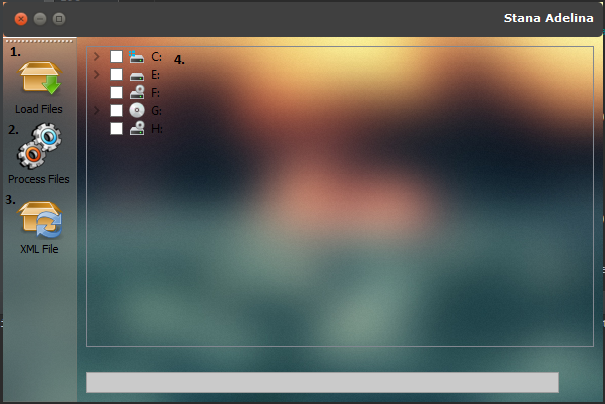
\includegraphics[width=\textwidth]{tool.png}
\caption{User interface}
\label{fig:figtool}
\end{figure*}

\tab For building the logical and structural dependencies the project root folder is needed. The tool offers a tree view of all the file system as shown in 4. of figure \ref{fig:figtool} . \\ The user does not have to select manualy each file, the selection of a folder implies the automatic selection of all subfolders and files. Also there is no need to select only the source code files, the tool processes all the files selected and only the ones with the accepted extensions are taken into consideration. To load all the files selected in the tool the button \textit{Load Files} needs to be pressed shown in 1. of figure \ref{fig:figtool} .

\section{Processing files}
\tab The next and final step to obtain the results is to press \textit{Process Files} button shown in 2. in figure \ref{fig:figtool} . The tool has a process bar wich shows to the user the percent of files processed as shown in figure \ref{fig:figloading} .

\begin{figure*}[h]
\centering
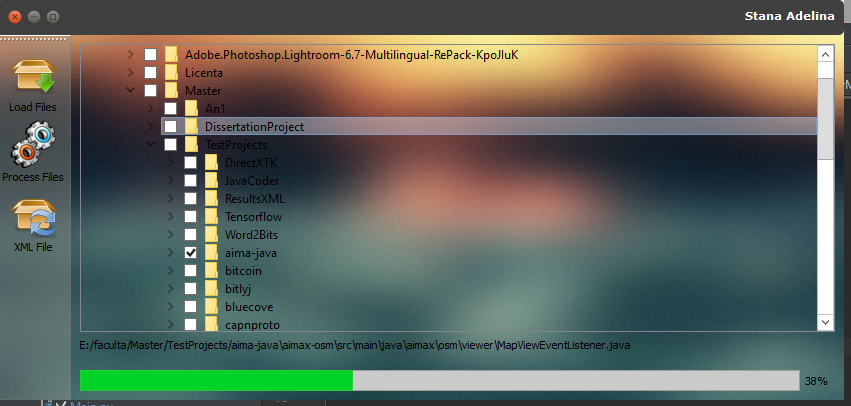
\includegraphics[width=\textwidth]{loading.png}
\caption{Loading files process bar}
\label{fig:figloading}
\end{figure*}

 This step implies the creation of XML files corresponding to the source code files , identifying the Git repository of the project, optaining all the structural and logical dependencies and their overlapings graphs .

\section{Load XML of previous run}
\tab Once the logical and structural dependencies are extracted the tool builds and saves a XML file with all the informations collected. So, if a project needs to be reanalysed, only the XML file needs to be uploaded. In this way a lot of time is saved since is no need to recolect data from source code files and commits. To perform this action the Load XML button (number 3. in figure \ref{fig:figtool} ) needs to be pressed and a file browse dialog will appear so the user can choose the file as shown in figure \ref{fig:figxmlload}.
\begin{figure*}[h]
\centering
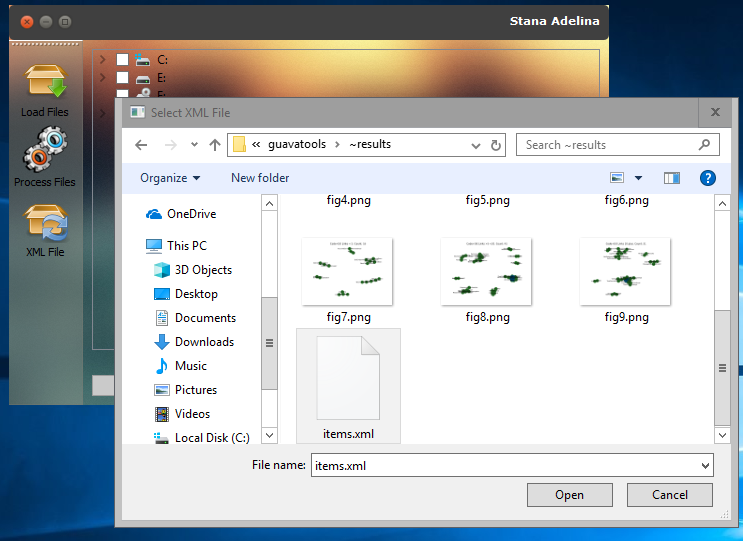
\includegraphics[width=\textwidth]{xmlload.png}
\caption{Loading a XML of a previous run.}
\label{fig:figxmlload}
\end{figure*}
\\
\tab The xml file is saved in the \textit{~results} folder created by the tool. The tool creates for each project analysed 3 folders , 2 temporary folders which are deleted after the process run and one results folder which is not deleted after the process run. The first temporary folder is the one that contains all the source code coresponing XML files , the second contains all the differences files extracted from the project commits. The last one is the \textit{~results} folder which contains all the graphics generated and the XML file with all the data extracted.
\\
\\
\\
\section{Output graphics}
 
\tab The output of the analysis made by the tool is represented as a series of graphics. Each graphic has in it's title the semnification of the displayed values and their counter (Figure \ref{fig:gitlinks}). For example for structural and logical dependencies found in files with less then 5 files changed the tool will display a graphic with the name "Overlapping structural and logical for more the 5 files changed . Counter : numberOfOverlaps" .
The tool will create graphics for the following casess: 
\begin{itemize}
  \item Structural dependencies found.
  \item Logical dependencies found in commits with less then 5 files changed.
  \item Logical dependencies found in commits with more then 5 files changed and less the 20.
  \item Logical dependencies found in commits with more then 20 files changed.
  \item The intersection of all the logical dependencies from all the 3 categories.
  \item The intersection between structural and logical dependencies found in commits with less then 5 files changed.
  \item The intersection between structural and logical dependencies found in commits with more then 5 files changed and less the 20.
  \item The intersection between structural and logical dependencies found in commits with more then 20 files changed .
  \item The intersection between structural dependencies and the intersection of all the logical dependencies from all the 3 categories .
\end{itemize}

Figure \ref{fig:gitlinks}
\begin{figure*}[h]
\centering
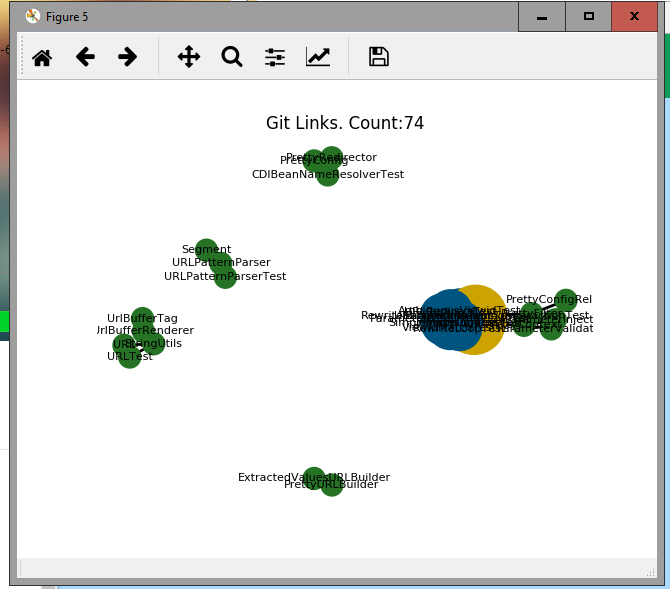
\includegraphics[width=\textwidth]{gitlinks.png}
\caption{Output graph from the analysis}
\label{fig:gitlinks}
\end{figure*}
